\chapter{Validierung}
%Überprüfen der Thesen
%    Szenarien mit erwarteten Ergebnissen vergleichen
%    Ergebnisse über Prototyp bestätigen
    
Um bewerten zu können, ob das entwickelte Programm den im Kapitel 4 genannten Anforderungen entspricht, wird in diesem Kapitel zur Validierung ein virtuelles Labor aufgebaut, dass \ac{IoT}-Client, einen Broker und natürlich den Proxy bereitstellt.

%Szenario, was mit dem Labor versucht wird zu erreichen.
Das Labor bildet die Kommunikation zwischen einem Sensor, welcher sich in der Glühbirne im Wohnzimmer des Nutzer befindet, und dem Broker des Herstellers. Der Sensor, im weiteren Client genannt, stellt dem Broker jede Sekunde den aktuelle Status zur Verfügung. Der Broker auf der anderen Seite erwartet den Status eines Clients und gleicht diese mit dem, vom Nutzer hinterlegten, Wunschwert ab. Anschließend sendet er bei einer Differenz zum Wunsch den neuen Wert los und bei einer Übereinstimmung einfach den gleichen Wert zurück.
%Erhält der Broker ein zu niedrigen Wert sendet er einen Befehl womit die Heizung die Leistung erhöht. Für den Fall, dass die aktuelle Temperatur höher als die eingestellte Temperatur ist, wird ein Befehl gesendet, wodurch die Heizung die Leistung reduziert.

\begin{figure}[h]%h=direkt danach t=top b=bottom
    \centering
    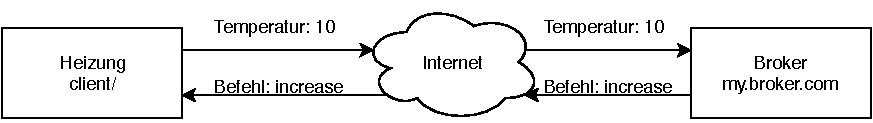
\includegraphics[width=14cm]{tex/bilder/6_validierung/Szenario1.pdf}
    \captionof{figure}{Darstellung des Szenarios}
    \label{fig:darstellung-szenario}
\end{figure}

\section{Laboraufbau}
    %Warum Virtualisierung/ Virtualisierte Umgebung
    Das Labor wird mithilfe der Virtualisierungslösung ESXi %\cite{https://www.vmware.com/de/products/esxi-and-esx.html}
    von VMware umgesetzt. Dadurch, dass alle Systeme und Applikationen in sogenannten Virtuellen Maschinen laufen sind sie, obwohl sie auf dem gleichen Gerät (Server) laufen können, voneinander unabhängig. Das bedeutet, dass ganze Systeme abgeschottet und auf \ac{VMDK}s gespeichert und somit auch sehr einfach gesichert oder untereinander ausgetauscht werden können. Durch die dynamische Verteilung von zum Beispiel CPU oder RAM ist ebenfalls eine effektivere Nutzung der Ressourcen möglich. Damit wird nur ein Server oder leistungsfähiger Computer benötigt um ganze Systemlandschaften und Netzwerke abzubilden. Des Weiteren ermöglicht es auch die hier durchgeführten Tests und somit Ergebnisse in der gleichen Umgebung durch die Bereitstellung der Dateien nachvollziehen zu können ohne selbst Arbeit und Zeit investieren zu müssen.
    %Warum mit ESXI
    ESXi wurde als Lösung gewählt, da bereits Wissen und Erfahrung im Umgang mit der Lösung vorhanden war. Zusätzlich stand ein Server mit benötigter Leistung bereits zur Verfügung was wodurch das Aufsetzen und Konfigurieren eines solchen oder ähnlichen Produkts nicht mehr nötig machte.
    
    Die folgenden Voraussetzungen sind notwendig um das Programm ausführen zu können.
    \begin{itemize}
        \item Betriebssystem: ab Windows 7, Linux mit Mono
        \item Abhängigkeiten: .NET Framework v4.6.1
        \item Speicher: 50 MB frei
        \item RAM: 100 MB frei
        \item Prozessor: 2 virtuelle Kerne  mit 2,0 Ghz
    \end{itemize}
    
    Die in diesem Szenario enthaltenen System sind die folgenden.
    
    \subsection{Virtualisierung der Geräte}
        \begin{enumerate}
            \item Der Client (die Heizung) ist wie folgt konfiguriert:
            \begin{itemize}
                \item Debian 9
                \item Ressourcen ?, 
            \end{itemize}
            Programme und Pakete
            \begin{itemize}
                \item Python 2.X
                \item pip Pakete ?
            \end{itemize}
            
            \item Der Broker (vom Hersteller) ist wie folgt konfiguriert:
            \begin{itemize}
                \item Debian 9
                \item Ressourcen ?, 
            \end{itemize}
            Programme und Pakete
            \begin{itemize}
                \item Python 2.X
                \item pip Pakete ?
            \end{itemize}
            
            \item Der Proxy, welcher die Kommunikation überwacht: 
            \begin{itemize}
                \item Microsoft Windows 10 Pro, Version, 10.0.17763 Build 17763
                \item Die CPU besteht aus vier virtuellen CPU Kernen.
                \item Es wurde der Maschine 8 GB \ac{RAM} zur Verfügung gestellt.
                \item 50 GB virtuelle Festplatte nach der \ac{VMDK} Format-Spezifikation für \ac{VM}s.
            \end{itemize}
            Frameworks:
            \begin{itemize}
                \item Microsoft Visual C++ 2008
                \item Microsoft Visual C++ 2017
                \item .NET Framework 4.6.1
            \end{itemize}
        \end{enumerate}
    
    \subsection{Netwerk}
    Netzwerk-Setup
    
    \subsection{Konfiguration der Software}
    %Konfiguration
    Das Projekt ist im Standard auf x86 Prozessoren ausgerichtet, kann allerdings bei Bedarf auch auf x64 Prozessoren durch Änderung der entsprechenden Einstellung in \ac{VS} geändert werden.
    Eine Unterstützung für weitere Architekturen ist nicht gegeben.
    Zusätzlich ist bei Ausführung der Anwendung ein privilegierter Account erforderlich um die Berichtigung für Zugriff auf die erforderlichen Port zu erhalten.
    Es werden Port 1883 für die Kommunikation mit dem \ac{MQTT}-Protokoll und Port 80 für die \ac{REST} Schnittstelle, welche auch die Weboberfläche bereitstellt, benötigt.
    Der Proxy ist ausschließlich über die Adresse \glqq 127.0.0.1\grqq{} oder \glqq localhost\grqq{} erreichbar, da keine Benutzerauthentifizierung implementiert wurde. Da eine unberechtigte Verwendung im lokalen Netz oder bei Bereitstellung über eine öffentlich erreichbare Adresse nicht ausgeschlossen werden kann, wird die Änderung auch nicht empfohlen. Sofern jedoch die Notwendigkeit bestehen sollte, ist es möglich die Adresse im Quellcode, durch die lokale IP-Adresse des Gerätes auf dem der Proxy läuft, auszutauschen um eine parallele oder externe Verwendung zu ermöglichen.
    
    
\section{Ausführung und Bewertung}
Was wird ausgeführt, welche Tests
Als erstes mit einem Client
    Intercepten: werden keine neuen rausgeschickt? werden sie im Web angezeigt?
    Modifizieren: können die im Web modifiziert werden?
    Speichern von Änderungen: können nach der Mod die auch gespeichert werden?
    Neue Nachrichten schicken: können neue geschickt werden?
Als zweites mit zwei Clients

\section{Performance}
    Hier wird die Performance des Proxys analysiert um Hinweise auf Skalierbarkeit und notwendige Ressourcen zu erhalten.
    Folgende Performance-Werte wurden mithilfe des Visual Studio Profilers auf der \ac{VM} Proxy erfasst.
    
    \begin{enumerate}
        \item Ohne Clients:
        Solange das Programm im Leerlauf arbeitet, also nur Events registriert sind die auf die Einwirkung anderer Komponenten warten, benötigt das Programm 19 MB \ac{RAM} und hat eine maximale CPU Auslastung von 1 Prozent.
        \item Mit einem Client:
        Sobald der erste Client sich verbunden hat, wir nur 1 MB mehr \ac{RAM} benötigt, was auf ein Gesamt von 20 MB kommt. Im Gegensatz dazu werden nun nach der ankommenden Nachricht vom \ac{IoT}-Client alle Funktionen des Programms ausgeführt. Dies führt zu einer Erhöhung beim Ausführen der Connect Funktion auf 20 Prozent und anschießend maximal 17 Prozent.
        \item Mit zwei Clients:
        Kommt nun ein weiterer Client dazu, sodass nun zwei Clients mit dem Proxy verbunden sind, steigt der \ac{RAM} Verbrauch weiterhin nur um 1 Prozent auf 21 MB an. Die maximale CPU Auslastung steigt jedoch auf 33 Prozent, was eine Steigerung um 95 Prozent darstellt. Dies ist unter anderem auf ein aktuelles Problem %\cite{https://github.com/Patrick-DE/MQTT-Proxy/issues/3}
        zurückzuführen was dazu führt, dass jeder Client die Antworten aller Clients an den Proxy schickt. Dies bedeutet, dass Antworten des externen Brokers doppelt erfasst und publiziert werden.
        Bei genauerer Analyse beider, am Anstiegen beteiligten Funktionen, ist zu erkennen, dass der größte Ressourcenverbrauch bei den folgenden Funktionen ist.
        \begin{itemize}
            \item Für 30 Prozent der maximalen CPU Auslastung des Programms ist die Connect Funktion verantwortlich. Die Connect Funktion wird aufgerufen, sobald sich ein \ac{IoT}-Client bei dem Proxy registriert. Sie hat mehrere Abhängigkeiten zu weiteren Funktionen die die Methode aufwändiger macht.  
            \item Für 57 Prozent der maximalen CPU Auslastung des Programms ist die Systemfunktion Console.WriteLine() Funktion verantwortlich. Da in diesem Programm viele Informationen an die Konsolenoberfläche zur Information an den Entwickler oder Nutzer weitergereicht werden ist dies die Hauptursache, dass das Programm die oben genannten CPU Auslastung aufweist. Zu bemerken ist jedoch, dass diese nur den maximalen Wert anzeigen, welcher nur vorhanden ist, wenn Nachrichten an den externen Broker weitergeleitet werden.
        \end{itemize}
    \end{enumerate}